\chapter{引言}
% 解释:RISC-V、开源处理器、高性能、虚拟化、虚拟化扩展
% 提及:云和数据中心领域是热的,在工业界有人不断尝试,是值得做的。
% 尽管该项目可能无法实现、但是需要去尝试、合并到工业界中。
% 以未来为切入点,画大饼。
% 历史片段

% 2018年11月8日,在网信办、中科院等多个国家部委支持和指导下,
% RISC-V中国联盟于浙江乌镇举行的第五届互联网大会上正式宣布成立。
% 从成立到现在的5年见,可以看见国内RISC-V相关产业在快速的发展。
% RISC-V是一个基于精简指令集原则的指令集架构,与x86、ARM架构是对应的关系。
% 首先,RISC-V与其他指令集最大的不同点在与开源性,即不需要收取高额的版权费,
% 相对的,x86和ARM指令集知识产权的公司均为国外公司,不利于我国实现关键芯片的自主可控。
% 因此,开源意味着自由、安全及可控。
% 其次,RISC-V还具有简洁、模块化的特点,
% 意味着轻量化、低功耗、小体积,因此非常适用于移动设备,以及在多场景的灵活适应性。
% 正是具有以上特点,在计算机体系结构领域,RISC-V受到了学术界和工业界的广泛瞩目。
% 短短六年,中国目前有300家以上公司在关注RISC-V或以RISC-V指令集进行开发。
% 从嵌入式到AI服务器,各种类别的RISC-V处理器核百花齐放。
% 我们有理由相信,未来RISC-V将在中国的芯片领域有更大的应用空间和市场份额。

% 中科院计算所研究员孙凝晖院士如此说道:“
% 开源模式不仅仅是一种商业模式,也是一种生态构建方法,是一种复杂系统开发方法。
% 更蕴含着一种精神。开源不仅仅公开源代码,更重要的是协作开发流程的建立与社区治理机制的建设。”

% 和中国知网上收录的关于RISC-V的文章在2018到2023年的平均增长比例达到了17.21\%和17.37\%

% RISC-V重要性,RISC-V是什么
% 虚拟化技术的重要性,什么是虚拟化技术
% RISC-V也在不断迈向虚拟化技术,这是十分必要的一件事
% 最后说出我们的工作内容,在这里不用说调试的问题


近年来在计算机体系结构的研究催生了一种名为RISC-V\cite{asanovic2014instruction}
的新型指令集架构(Instruction Set Architecture,ISA)。
RISC-V凭借其开源、简洁、模块化的特性,受到了学术界和工业界的广泛瞩目。
首先,RISC-V与其他指令集最大的不同点在于开源性,即不需要收取高额的版权费,
相对的,x86和ARM指令集知识产权的公司均为国外公司,不利于我国实现关键芯片的自主可控。
因此,开源意味着自由、安全及可控。同时,RISC-V还具有简洁、模块化的特点,
这意味着轻量化、低功耗、小体积,因此非常适用于移动设备,以及在多场景的灵活适应性。
从SiFive推出的面向自动驾驶的芯片\cite{sifive-automotive},
到阿里巴巴达摩院的玄铁RISC-V系列处理器\cite{xuantie}。
RISC-V在嵌入式领域中,已经逐渐进入由ARM、x86等主流计算机架构垄断的芯片市场。

另一方面,虚拟化技术作为计算机科学领域的一项关键技术,为云数据中心提供的各类服务构建了核心的技术框架。
通过在计算机硬件上创建一个抽象层,虚拟化技术能够将单台计算机的硬件分成多个虚拟计算机。
每个虚拟机能够运行自己的操作系统,和其他虚拟机相互独立,同时又能被简单且可复现地构建、销毁。
这些优势与云计算的发展方向和对灵活IT解决方案的需求十分契合,真正改变了过去传统的基于物理机的运营模式。
随着服务器虚拟化已成为一种常见做法,许多企业已从物理现场数据中心转向虚拟化数据中心解决方案。
对于运营商而言,它能减少管理开支、停机时间,增强灾难恢复情况下的弹性,更充分利用硬件资源以提高效率和生产力。
对于用户而言,能够在需要时仅购买所需的计算资源,并随着工作负载的增长经济实惠地扩展这些资源。
随着近年来云数据中心及云服务提供商的快速发展,从初期的虚拟机与容器技术,
到新兴的函数即服务(Function as a Service, FaaS)与无服务器计算(Serverless)模式,
均展现出了强烈的市场需求和广阔的发展潜力。
这一趋势不断促进虚拟化技术的进步与创新,
处理器芯片行业的主要参与者开始在主流计算架构中引入硬件虚拟化支持以加速虚拟化软件的运行,
例如,Intel VT\cite{intel-VT2005Computer}以及ARM的VE扩展\cite{armve2018}。
自然的,RISC-V也希望能够处理云数据中心的需求,因此也在积极的推进虚拟化的硬件扩展的相关研究。

\begin{figure}[htbp]
\centering
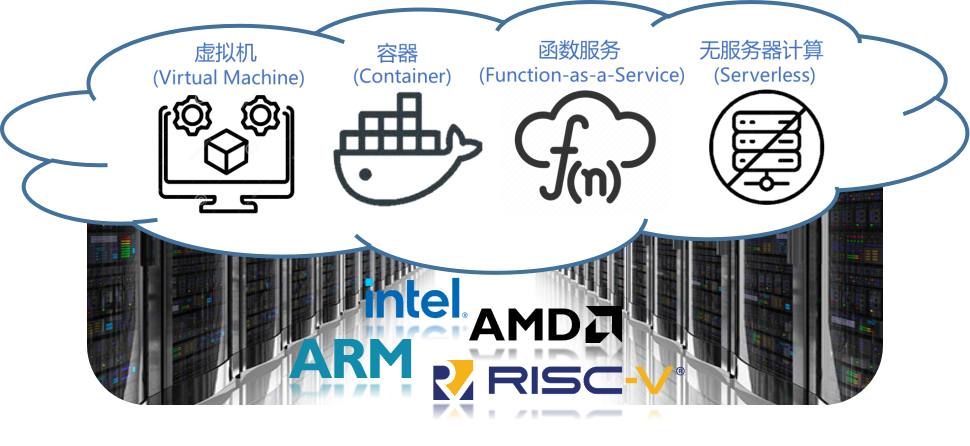
\includegraphics[scale=0.5]{virtual.png}
\caption{云数据中心在不同指令集架构的发展}
\end{figure}

然而,关于RISC-V虚拟化的研究尚处于起步阶段,还有巨大的研究空间。
2017年,RISC-V官方提出了虚拟化扩展的概念,规定了支持虚拟化的处理器需要额外添加的特权级和指令等。
截至2021年12月,虚拟化扩展才被正式批准。
同一年,加州大学的伯克利分校迈出了虚拟化扩展硬件实现的第一步。
他们研发了Rocket Chip\cite{itco2022rocket},一个开源的RISC-V顺序流水线处理器,
在其上实现了完整的虚拟化扩展,并进行了一系列虚拟化相关的评测。
但是,在真实应用场景下,处理器的情况会更为复杂,
多核乱序的高性能处理器才是虚拟化服务器的主流。
因此,本文计划瞄准高性能RISC-V处理器的虚拟化扩展实现,开展从硬件扩展到软件适配的全系统评测的研究。

高性能RISC-V处理器的一个典型代表便是中国科学院计算技术研究所牵头发起的“香山”项目。
作为目前国际上性能最高的开源高性能RISC-V处理器核的同时,
“香山”致力成为一个开源的工业级别处理器,并成为面向世界的体系结构创新开源平台。
计算所研究员孙凝晖院士对开源精神表示:“
开源模式不仅仅是一种商业模式,也是一种生态构建方法,是一种复杂系统开发方法。
更蕴含着一种精神。开源不仅仅公开源代码,更重要的是协作开发流程的建立与社区治理机制的建设。”
“香山”始终坚持、坚定地开源所有的设计、验证、基础工具代码,对来自社区的贡献始终表示欢迎。
因此,十分适合用于高性能RISC-V处理器的虚拟化扩展研究。

本文的尝试研究如图\ref{fig:level}的虚拟化系统。
首先,在底层的硬件,需要为“香山”处理器的“南湖”架构——一个用于学术研究的稳定版本,添加虚拟化扩展。
第二,在扩展的处理器中运行虚拟机管理系统。
本文选用经典的Type2虚拟机管理系统Linux-KVM\cite{kvm:H-ext},并尝试在此基础上启动虚拟机。
最后,尝试在整个软硬件系统中,使用FPGA加速仿真平台进行系统级的评测和调试。

在处理器微架构方面,本文扩展了“香山”的特权管理单元和内存管理单元。
特别是虚拟内存部分,通过添加第二阶段地址翻译单元、实现了第二阶段页表翻译。
还通过复用二级页表缓存、猝发传输获取页表、压缩一级页表缓存表项等的微架构加快了翻译速度,提高了吞吐量。
在虚拟机管理软件的适配方面,本文在虚拟化扩展的“香山”中启动了Linux,并尝试使用KVM启动虚拟机。
在系统级评测中,本文完成了针对主机系统的性能评测,以及软硬件联合调试工具的创新研究。
由于在对虚拟机系统的进行性能评测时,处理器潜在的错误导致虚拟机启动失败,
因此,本文探索了通过使用体系结构检查点来跳过启动操作系统的纯软件加速手段,
和FPGA仿真加速平台联合差分测试框架的调试手段。

\begin{figure}[htbp]
    \centering
    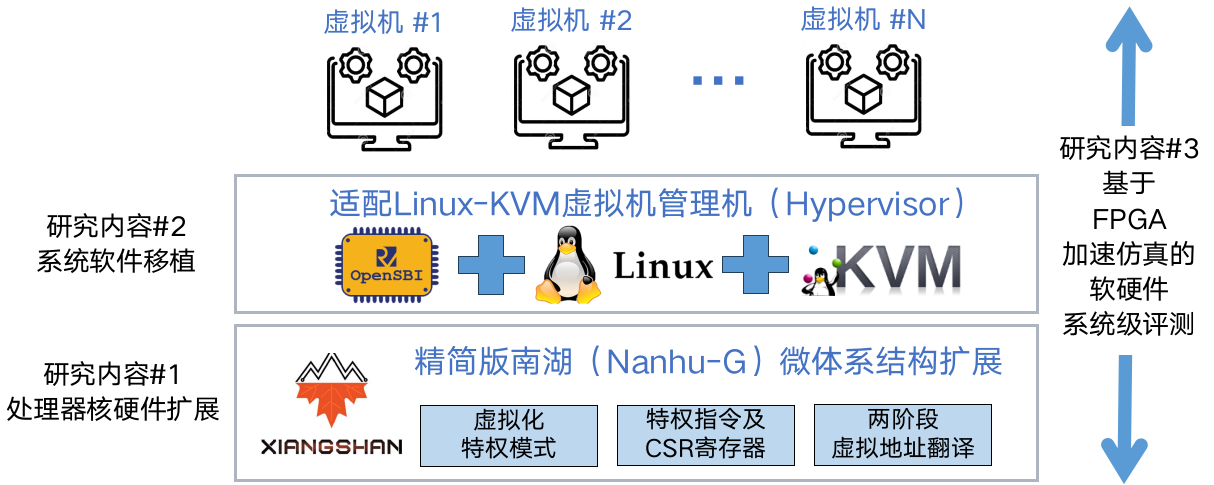
\includegraphics[scale=0.45]{level.png}
\caption{虚拟化体系结构与本文研究内容}
    \label{fig:level}
\end{figure}
